      
               
                \begin{ledgroupsized}[r]{120mm}
                \footnotesize 
                \pstart                
                \noindent\textbf{\"{U}berlieferung:}   
                \pend
                \end{ledgroupsized}
            
              
                            \begin{ledgroupsized}[r]{114mm}
                            \footnotesize 
                            \pstart \parindent -6mm
                            \makebox[6mm][l]{\textit{L}}Konzept: LH XXXVII 3 Bl. 134\textendash 135. 1 Bog. 2\textsuperscript{o}. 2 S. zweispaltig auf Bl. 135. Die verbleibenden Seiten zu N. 49\raisebox{-0.5ex}{\notsotiny 3} geh\"{o}rig. Auf Bl. 135 r\textsuperscript{o} unsere Zeichnungen fig. 1\textendash3. Eine vierte von Leibniz nicht bezeichnete und gestrichene Figur wird im Folgenden nicht berücksichtigt, da es sich um einen ersten Versuch zu fig. 2 handelt. Die Zeichnungen wurden in N. 51 noch einmal verwendet und zu diesem Zweck in fig. 2 bis fig. 4 umbenannt. Daraus ergibt sich die Reihenfolge der St\"{u}cke. Bl. 135 r\textsuperscript{o} ist mit Ausnahme der \"{U}berschrift von Leibniz vollst\"{a}ndig gestrichen worden. Die Streichung erstreckt sich bis auf den ersten Abschnitt von Bl. 135 v\textsuperscript{o}. Wir behandeln diese Textpassagen der \"{U}bersichtlichkeit halber wie g\"{u}ltigen Text und setzen sie in Kleindruck.\\Cc 2, Nr. 491 G tlw. \pend
                            \end{ledgroupsized}
                \vspace*{8mm}
                \pstart 
                \normalsize
            \selectlanguage{french}\begin{center}[135 r\textsuperscript{o}] Experiences, \`{a} faire en\\cette matiere:\edlabel{mati135r1}\end{center} %\pend 
         %   \pstart  
            \edtext{\edlabel{mati135r2}}{\lemma{}\xxref{mati135r1}{mati135r2}\Afootnote{matiere: \textbar\ \textso{Experience 1.} S\c{c}avoir la hauteur du tuyau  plein de Mercure purg\'{e}\protect\index{Sachverzeichnis}{mercure!purg\'{e}} capable \`{a} le faire tomber pour faire cela simplement   \textbar\ et   \textbar\ pour \textit{ erg.}\ \textbar\  purger le Mercure\protect\index{Sachverzeichnis}{mercure} parfaitement avec peu de peine \textit{ erg.}\ \textbar\ , voicy la maniere,  \textit{ (1) }\ prennez  \textit{(a)}\ le plus long \textit{(b)}\ plusieurs tuyaux propres pour des barometres\protect\index{Sachverzeichnis}{barom\`{e}tre|textit}, \`{a} l'ordinaire, et \textit{ (2) }\ faites l'experience de Torricelli en plusieurs tuyaux, et quand vous croyez que quelque air sortit du Mercure s'est repandu dans le vuide tourn\'{e}z les tuyaux alors l'air qui est dans le vuide sera contraint de monter, et de sortir par l'ouuerture du tuyau. Si vous continuez cela plusieurs fois, le Mercure sera bien purg\'{e}. Alors versez le Mercure purg\'{e}  de plusieurs  \textit{(a)}\ petits tuyaux dans un grand \textit{(b)}\ tuyaux ordinaires dans un autre aussi  \textit{(aa)}\ grand \textit{(bb)}\ long que vous le pouuez trouuer pour essayer si l'on peut arriver \`{a} la derniere hauteur.   \textbar\ Alors on trouvera aussi, si en chargeant le tuyau plus que l'attachement ne peut supportant, le surplus tombe seulement, ou le tout. \textit{ erg.}\ \textbar\  \textit{ gestr.}\ \textbar\ \textso{Experience} \textit{ L}}}
          %  \clearpage
            \footnotesize \textso{Experience 2}\textsuperscript{me}\textso{. }\edtext{\textso{Trouuer}}{\lemma{2\textsuperscript{me}.}\Afootnote{ \textit{ (1) }\ \textso{S\c{c}avoir} \textit{ (2) }\ \textso{Trouuer} \textit{ L}}}\textso{ la force necessaire pour }\edtext{\textso{separer}}{\lemma{\textso{pour}}\Afootnote{ \textit{ (1) }\ \textso{desunir} \textit{ (2) }\ \textso{separer} \textit{ L}}}%\linebreak
            \textso{ deux placques }\edtext{\textso{d'une largeur considerable, et de toutes sortes de 
         %   \clearpage
            matieres}}{\lemma{}\Afootnote{\textso{d'une largeur } \textit{ (1) }\ \textso{autant considerable qu'il est possible} \textit{ (2) }\ \textso{considerable, et de toutes sortes de matieres} \textit{ erg.} \textit{ L}}}\textso{ dans }\edtext{\textso{l'air libre aussi bien que}}{\lemma{\textso{dans}}\Afootnote{ \textit{ (1) }\ \textso{le libre et} \textit{ (2) }\ \textso{l'air libre aussi bien que} \textit{ L}}}\textso{ dans le vuide.} \edtext{L'usage de cette experience est, pour s\c{c}avoir si dans l'air libre l'union des placques est plus forte qu'\`{a} raison de la seule pression de l'atmosphere}{\lemma{\textso{vuide.}}\Afootnote{ \textit{ (1) }\ Dans l'air libre on peut attacher   \textbar\ librement \textit{ erg.}\ \textbar\ des poids jusqu'  \textit{(a)}\ \`{a} la desunion \textit{(b)}\ \`{a} ce qu'ils desunissent les \textit{ (2) }\ Les poids estant attachez au milieu ou aux costez des deux placques: mais dans le vuide\protect\index{Sachverzeichnis}{vide|textit}, il faut un grand Recipient si les placques sont fort larges, pour placer les poids, mais si la place est trop petite, on les peut faire la desunion par un ressort cach\'{e} \`{a} propos \textit{ (3) }\ L'usage de cette  \textit{(a)}\ force \textit{(b)}\ experience est,   \textbar\ pour \textit{ erg.}\ \textbar\ s\c{c}avoir [...] l'atmosphere \textit{ L}}} \edtext{comme l'experience du Mercure purg\'{e}\protect\index{Sachverzeichnis}{mercure!purg\'{e}} suspendu dans l'air libre, d'une hauteur de 70 pouces le semble inferer. Car puisque l'union des placques persiste aussi bien dans le vuide\protect\index{Sachverzeichnis}{vide}, que celle de la liqueur purg\'{e}e\protect\index{Sachverzeichnis}{liqueur!purg\'{e}e}, elle semble estre d'un même principe. Quoyque M. Guericke\protect\index{Namensregister}{\textso{Guericke} (Gerickius, Gerick.), Otto v. 1602\textendash 1686} pretend d'avoir calcul\'{e} qu'il faut justement une force egale \`{a} celle de la colomne d'air pour separer ces deux placques}{\lemma{comme}\Afootnote{[...] inferer.  \textbar\ Car [...] semble  \textit{ (1) }\ provenir \textit{ (2) }\ estre d'un même principe. \textit{ erg.}\ \textbar\  Quoyque [...] placques \textit{ erg.} \textit{ L}}};\edtext{}{\lemma{placques;}\Bfootnote{\textsc{O. v. Guericke,} \cite{00055}\textit{Experimenta nova}, Amsterdam 1672, S.~101\textendash103.\hspace{2cm} }} et \edtext{on remarquera aussi}{\lemma{}\Afootnote{on remarquera aussi \textit{ erg.} \textit{ L}}} si l'union dans l'air libre est plus forte que dans le vuide; et de combien, \edtext{et si elle est plus au moins forte, dans des liqueurs, comme eau, huyle, que dans l'air (la pesanteur des liqueurs estant soubstraite,) pour juger si cette union vient du mouuement de la liqueur ambiante. Item ce qui arrive quand les superficies interieures des placques devant que d'estre jointes ont est\'{e} moûilleës, comme d'eau ou d'esprit de vin, si la separation des placques produit quelque son hors du vuide ou dans le vuide.}{\lemma{combien,}\Afootnote{ \textit{ (1) }\ il faut conferer cela avec l'objection 5\textsuperscript{me}. \textit{ (2) }\ et si  \textit{(a)}\ l'on trouveroit \textit{(b)}\ elle [...] vuide. \textit{ L}}}
            \pend
%             \begin{center}
%          % \begin{wrapfigure}{l}{0.4\textwidth}                    
%                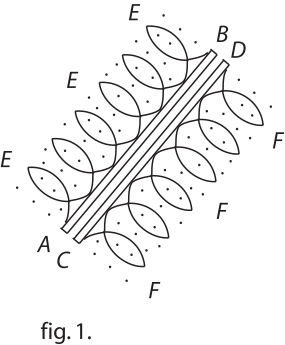
\includegraphics[width=0.4\textwidth]{images/37_3_135r1}
%                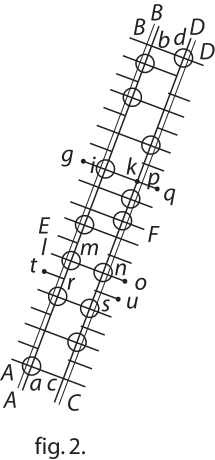
\includegraphics[width=0.3\textwidth]{images/37_3_135r2}\\
%                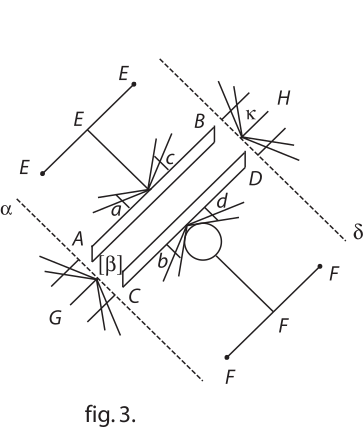
\includegraphics[width=0.5\textwidth]{images/37_3_135r3}
%                \newpage  
%             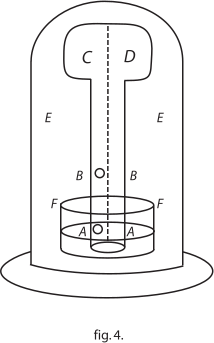
\includegraphics[width=0.4\textwidth]{images/37_3_135r4}
%\end{center}             
\pstart
             \footnotesize\textso{Experience 3}\textsuperscript{me}. S\c{c}avoir si une liqueur purg\'{e}e\protect\index{Sachverzeichnis}{liqueur!purg\'{e}e} s'attache dans le tuyau non seulement en-haut, mais même aux costez. Et par consequent si le haut du matras \textit{CD} estant ouuert \edtext{ou rompu}{\lemma{}\Afootnote{ou rompu \textit{ erg.} \textit{ L}}}, apres qu'il  a demeur\'{e} longtemps dans le vuide tout plein, exp. 16. l'eau tombe. On pourra dire pourtant que \edtext{le peu de l'air qui reste dans le Recipient y pouuant arriver que}{\lemma{que}\Afootnote{ \textit{ (1) }\ cela arrive que \textit{ (2) }\ le [...] que \textit{ L}}} feroit cet effect, comme la petite bulle dans l'objection 6\textsuperscript{me}. Il merite pourtant de l'essayer. Mais il y a une autre experience pour cet effect; \edtext{qui n'est pas expos\'{e}e \`{a} cette replique}{\lemma{}\Afootnote{qui [...] replique \textit{ erg.} \textit{ L}}}. Car comme le siphon \`{a} jambes inegales tombe dans le vuide\protect\index{Sachverzeichnis}{vide}, on le pourra faire recommencer, apres que l'eau purg\'{e}e y a est\'{e} longtemps en repos. Le même se fera en faisant jouer une pompe\protect\index{Sachverzeichnis}{pompe} apres un long repos. \edtext{On peut commencer le mouuement de la pompe\protect\index{Sachverzeichnis}{pompe} ou du siphon\protect\index{Sachverzeichnis}{siphon} dans l'air libre, et il pourra durer jusque \`{a} ce que le Recipient soit assez vuide, pourveu que le mouuement soit tard.}{\lemma{}\Afootnote{On peut commencer  \textbar\ par dehors, et pendant que \textit{ gestr.}\ \textbar\   le mouuement [...] tard. \textit{ erg.} \textit{ L}}}\pend \pstart \footnotesize\textso{Experience 4}\textsuperscript{me}. \edtext{S\c{c}avoir si les liqueurs dans lesquelles on met les deux}{\lemma{4\textsuperscript{me}.}\Afootnote{ \textit{ (1) }\ On peut eprouuer si les deux \textit{ (2) }\ S\c{c}avoir [...] deux \textit{ L}}} placques unies, apportent quelque changement outre celuy de leur pesanteur. On peut eprouuer cela dans le vuide et hors du vuide, il faut substraire la pression de la colomne de la liqueur\protect\index{Sachverzeichnis}{liqueur}, et afin qu'elle ne soit pas considerable, il ne faut pas enfoncer dedans que tant soit peu les dites placques, si les liqueurs\protect\index{Sachverzeichnis}{liqueur} (leur pasanteur estant soustraite,) n'y apportent point de changement